% I actually like landscape documents . Forces you to be concise
\documentclass[a4paper,12pt,landscape,twocolumn]{book}
\usepackage[a4paper,inner=2cm,outer=2cm,top=2cm,bottom=2cm]{geometry}

% Basic Packages and settings i prefer
\usepackage{blindtext}
\linespread{1.3} % I like thocc linespacing in my articles
\setlength{\columnsep}{1.3cm} % And column as wide as yo mama

% Other Packages you would most probably need
\usepackage{microtype}
\usepackage{graphicx}
\usepackage{wrapfig}
\usepackage{index}
\usepackage[english]{babel} % load index before babel

% Sometimes i feel fancy
\usepackage{fancyhdr}



\makeindex
\begin{document}

	% Make Title Page
	\title{\Large{Latex 'Lahtec' Tutorial}}
	\author{By Adi}
	\date{Apr 2018}
	\maketitle
	\let\cleardoublepage\clearpage % clears weird empty pages

	% Make Contents Page
	\tableofcontents
	\pagenumbering{roman}
	\setcounter{page}{2}

	% Set your headers and footers here
	\pagestyle{fancy}
	\fancyhf{} % init
	% left header
	\lhead{\itshape Chapter \thechapter \chaptermark}
	% right header
	\rhead{\itshape Section \thesection \sectionmark}

	% right footer
	\rfoot{\thepage}

	\setlength{\headheight}{14.5pt}
	
	% Lorem Ipsum your pages to test your layout
	\chapter{First Chapter}
	\blindmathtrue
	\blindtext[5]
	\section{First Section}
	\blindtext[3]
	\section{Second Section}
	\blindtext[2]


	\chapter{Second Chapter}
	\blindmathtrue
	\blindtext[5]
	\section{First Section}
	\blindtext[3]
	\section{Second Section}
	\blindtext[2]

	% Add some pictures just for demo purposes
	\begin{figure}[ht]
		\centering
		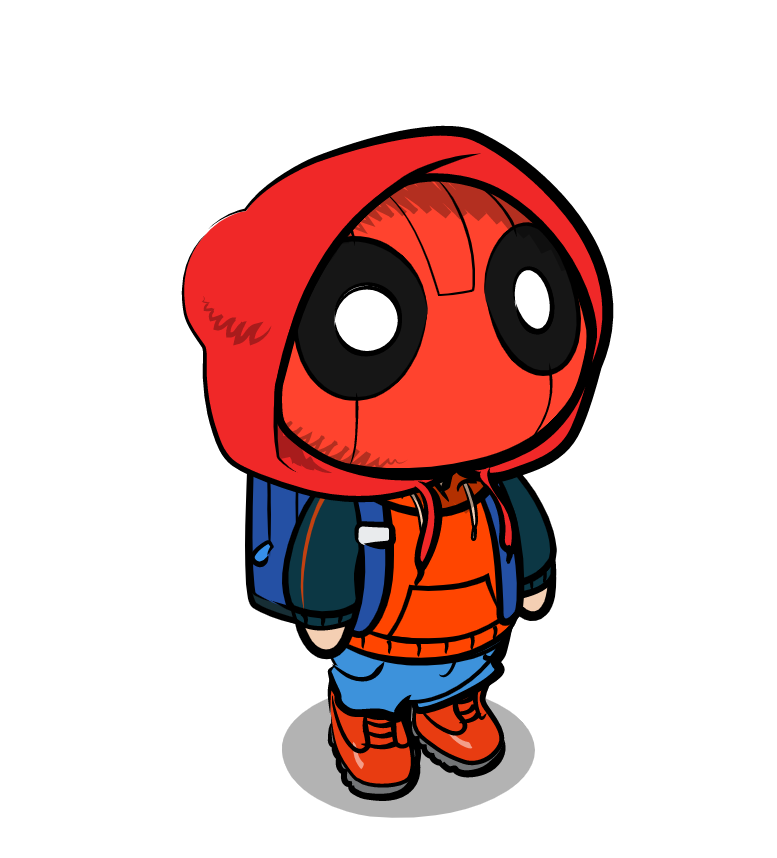
\includegraphics[width=3cm,height=4cm]{spiderman.png}
		\caption{\itshape Your Friendly Neighbourhood spiderman}\label{fig:spiderman}
	\end{figure}
	\blindtext[5]

	\chapter{Third Chapter}
	\blindmathtrue
	\blindtext[5]
	\section{First Section}
	\blindtext[3]
	\begin{itemize}
		\item \blindtext
		\item \blindtext
		\item \blindtext
	\end{itemize}
	\section{Second Section}
	\blindtext[2]
\end{document}

